\documentclass{standalone}
\usepackage{tikz}
\usetikzlibrary{calc}

\begin{document}
	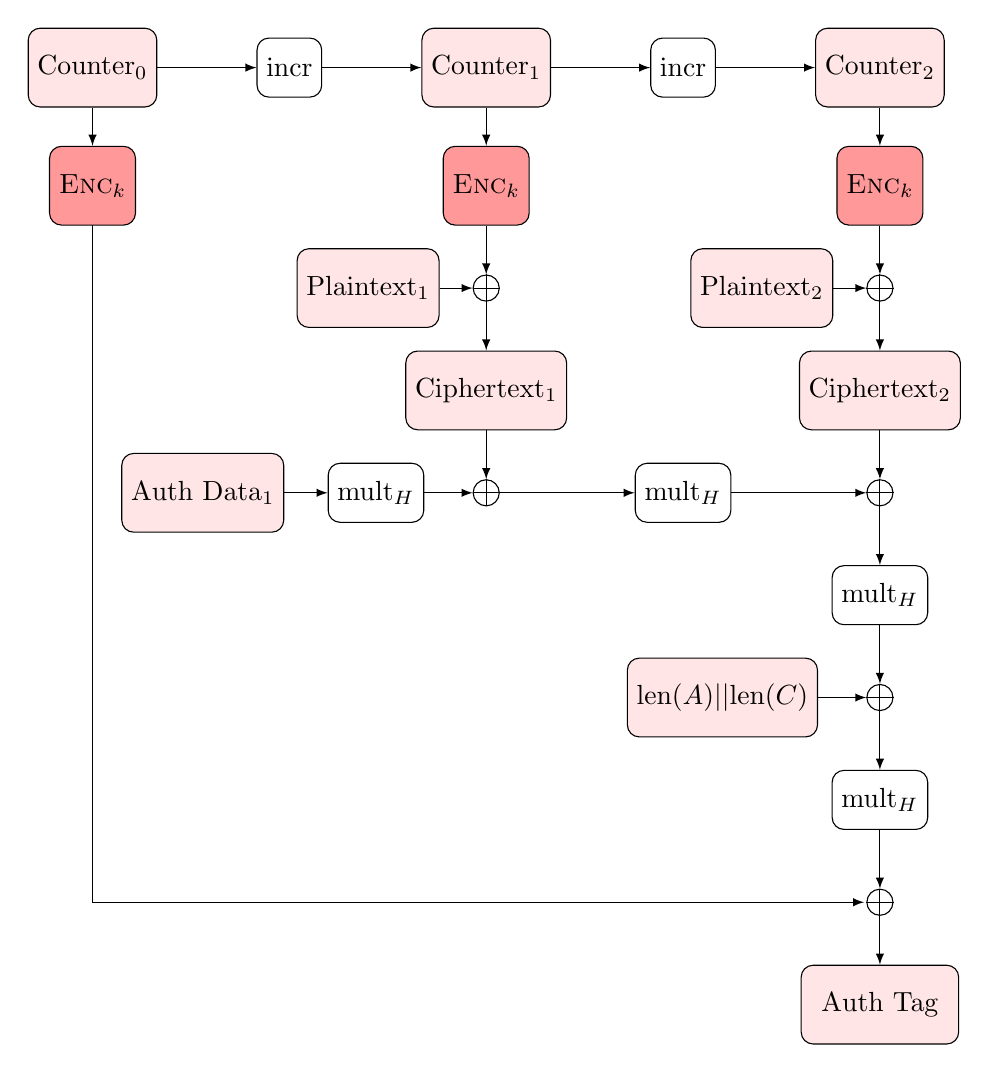
\begin{tikzpicture}
		
		\foreach \x in {0,1,2} {
			\node (f\x) at ($\x*(5cm,0)$) [minimum size=0.75cm, minimum height=1.0cm, rounded corners=1ex,fill=red!10,draw] {Counter$_\x$};
			\node (c\x) [minimum size=0.75cm, minimum height=1.0cm, rounded corners=1ex,fill=red!40,draw] [below of=f\x, node distance=1.5cm] {{\sc Enc}$_k$};
			\draw[-latex] (f\x) -- (c\x);
		}
		
		\node (incr1) [minimum size=0.5cm,minimum size=0.75cm, rounded corners=1ex,draw][right of=f0, node distance=2.5cm] {incr};
		\node (incr2) [minimum size=0.5cm,minimum size=0.75cm, rounded corners=1ex,draw][right of=f1, node distance=2.5cm] {incr};
		\draw[-latex] (f0) -- (incr1);
		\draw[-latex] (incr1) -- (f1);
		\draw[-latex] (f1) -- (incr2);
		\draw[-latex] (incr2) -- (f2);
		
		\foreach \x in {1, 2} {
			\node (p\x) [below of=c\x, node distance=1.3cm, circle, draw] {};
			\node (m\x) [below of=p\x, node distance=1.3cm, minimum size=0.75cm, minimum height=1.0cm, rounded corners=1ex, fill=red!10, draw] {Ciphertext$_\x$};
			\node (k\x) [below of=m\x, node distance=1.3cm, circle, draw] {};
			\draw[-] (p\x.north) -- (p\x.south);
			\draw[-] (p\x.east) -- (p\x.west);
			\draw[-] (k\x.north) -- (k\x.south);
			\draw[-] (k\x.east) -- (k\x.west);
			\draw[-latex] (p\x) -- (m\x);
			\draw[-latex] (m\x) -- (k\x);
		}
		
		\node (b1) [right of=k1, node distance=2.5cm, minimum size=0.75cm, rounded corners=1ex, draw] {mult$_H$};
		\node (b2) [below of=k2, node distance=1.3cm, minimum size=0.75cm, rounded corners=1ex, draw] {mult$_H$};
		\draw[-latex] (k1) -- (b1);
		\draw[-latex] (k2) -- (b2);
		
		\draw[-latex] (c1) -- (p1);
		\draw[-latex] (c2) -- (p2);
		\node (iv1) [left of=p1, node distance=1.5cm, minimum size=0.75cm, minimum height=1.0cm, rounded corners=1ex, fill=red!10, draw] {Plaintext$_1$};
		\draw[-latex] (iv1) -- (p1);
		\node (iv2) [left of=p2, node distance=1.5cm, minimum size=0.75cm, minimum height=1.0cm, rounded corners=1ex, fill=red!10, draw] {Plaintext$_2$};
		\draw[-latex] (iv2) -- (p2);
		
		\node (bb) [left of=k1, node distance=1.4cm, minimum size=0.75cm, rounded corners=1ex, draw] {mult$_H$};
		\node (ad) [left of=bb, node distance=2.2cm, minimum size=0.75cm, minimum height=1.0cm, rounded corners=1ex, fill=red!10, draw] {Auth Data$_1$};
		
		\draw[-latex] (bb) -- (k1);
		\draw[-latex] (ad) -- (bb);
		
		\node (circ1) [below of=b2, node distance=1.3cm, circle, draw] {};
		\node (bbb) [below of=circ1, node distance=1.3cm, minimum size=0.75cm, rounded corners=1ex, draw] {mult$_H$};
		\node (circ2) [below of=bbb, node distance=1.3cm, circle, draw] {};
		\node (at) [below of=circ2, node distance=1.3cm, minimum size=2cm, minimum height=1.0cm, rounded corners=1ex, fill=red!10, draw] {Auth Tag};
		\node (concat) [left of=circ1, node distance=2.0cm, minimum size=0.75cm, minimum height=1.0cm, rounded corners=1ex, fill=red!10, draw] {len($A$)$||$len($C$)};
		
		\draw[-latex] (b2) -- (circ1);
		\draw[-latex] (circ1) -- (bbb);
		\draw[-latex] (bbb) -- (circ2);
		\draw[-latex] (circ2) -- (at);
		\draw[-] (circ1.north) -- (circ1.south);
		\draw[-] (circ1.east) -- (circ1.west);
		\draw[-] (circ2.north) -- (circ2.south);
		\draw[-] (circ2.east) -- (circ2.west);
		\draw[-latex] (concat) -- (circ1);
		\draw[-latex] (b1) -- (k2);
		\draw[-latex] ($(c0)+(0,-0.5cm)$) |- ($(circ2) + (-0.2cm,0cm)$);
		
	\end{tikzpicture}
\end{document}